\section{Runtime Architecture and Research Context}
\label{sec:runtime}
\subsection{Execution as a stateful transaction}
A speculative iteration advances a committed prefix through drafting, target verification and reconciliation. The draft proposes up to $k$ tokens; the target evaluates the pending token and proposal positions, often in a caller batch containing several tokens. Acceptance, correction and a possible bonus token determine the committed output. Rejected positions must be removed or reconciled before the next iteration, and stopping follows the registered EOG and cap rule. Figure~\ref{fig:architecture} connects these operations to the state and phase controls studied here.

Target and draft retain distinct state (Figure~\ref{fig:architecture}A). KV ownership, logical positions, pending logits or tokens, sampler history and loop counters connect successive calls. A token can already be sampled and accepted into the sampler while still awaiting evaluation into the cache. Repeating or omitting either event changes the transaction. The early intervention frontends therefore preserve pending and sampler state as well as KV. The later B570 candidate binds phases within one target context and live sampler; the measured RTX candidate uses no state transplant.

\begin{figure*}[t]
\centering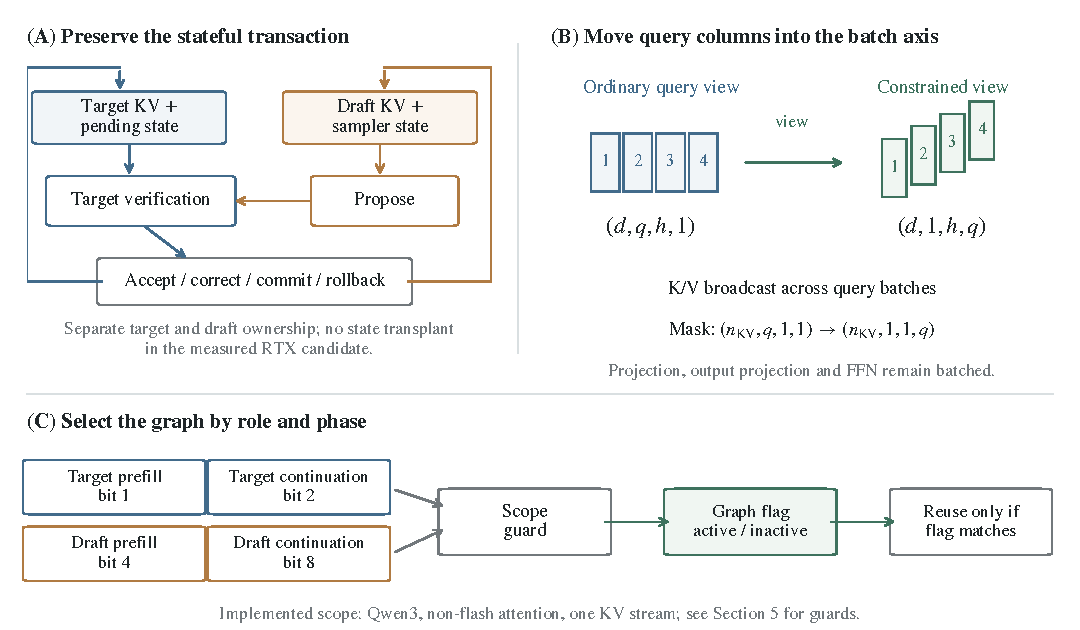
\includegraphics[width=\linewidth]{figures/figure_1_architecture.pdf}
\caption{State ownership and implemented consistency controls. (A) Target and draft keep distinct state through proposal, verification and reconciliation. (B) The RTX query view moves query columns into the batch axis while retaining batched projection and FFN work; numbered tiles are illustrative. (C) Role and phase select the query-batch graph flag, which must also match for topology reuse. The measured RTX candidate uses no state transplant. Section~\ref{sec:repair} defines the transformation and its implementation guards.}
\label{fig:architecture}
\end{figure*}

Microbatch capacity UB limits how the backend partitions a caller batch. It is distinct from $k$, the occupied query count and the frontend's output reservation. A UB2 caller may contain only one continuation token; increasing $k$ can reduce caller count while increasing the number of micrographs; changing output reservation can alter the recipe without changing UB. These distinctions are needed to interpret both diagnostic crosses and performance counters.

The implementations use pinned llama.cpp releases and private frontends~\cite{llamacpp}. The late RTX path uses Qwen3-8B and Qwen3-0.6B~\cite{qwen3}, both Q8\_0, with non-flash CUDA attention. Its transformation uses existing ggml views and operations, with no new CUDA arithmetic kernel or acceptance rule. B570 uses Vulkan and a distinct phase-binding frontend. Historical Metal and OpenVINO cases retain their own contracts. Because hardware, backend and frontend vary together, these cases compare execution designs rather than hardware alone.

\subsection{Reference preservation and determinism}
Our requirement fixes an ordinary path and an output endpoint. A matching token sequence may still have different logits or cache values, while a repeat-stable candidate can consistently disagree with the reference. Numerical-consistency work explains how execution shapes and reductions affect this distinction. Batch-invariant inference constrains reduction strategies across batches~\cite{thinkingmachines}. LLM-42 combines decode--verify--rollback, padded verification shapes and replacement of decoded KV entries with verifier entries; it permits different consistent strategies for prefill and decode~\cite{llm42}. Stage-Replay examines fixed-prefix precision controls and bidirectional cache transplantation~\cite{stagereplay}. Vosti specifies and verifies deterministic system behavior~\cite{vosti}, and MarginGate uses margin-triggered verification with repair of confirmed mismatches~\cite{margingate}.

Our implementation uses these established consistency and verification principles. Its additional evidence links natural donor-state diagnosis to a concrete query-layout and phase design, followed by finite native-output qualification and paid comparisons. Table~\ref{tab:related} summarizes this scope. We do not implement a same-contract comparison with LLM-42, Stage-Replay or Vosti, so the results establish no speed or preservation advantage over those methods.

\begin{table*}[t]\centering\small
\caption{Research context and additional evidence in this study. The cited methods are not same-contract performance baselines.}
\label{tab:related}
\begin{tabularx}{\linewidth}{@{}p{.23\linewidth}XX@{}}\toprule
Prior work & Established basis & Additional evidence here\\\midrule
Batch-invariant inference; LLM-42~\cite{thinkingmachines,llm42} & Reduction/shape consistency; verified tokens and KV reconciliation & Qwen3 query views and phase dispatch, finite qualification, and ordinary/matched paid costs\\
Stage-Replay; Vosti~\cite{stagereplay,vosti} & Fixed-prefix state intervention; specified system determinism & Natural donor $\times$ current-recipe crosses with shams; output qualification in a tested implementation family\\
Consumer cost anatomy; Performance or Illusion?~\cite{lossless,illusion} & Backend verification cost and limits of performance proxies & Qualified fixed-UB width failure and separation of target-path from speculative request gains\\\bottomrule
\end{tabularx}
\end{table*}

\subsection{Performance and heterogeneous execution}
Heterogeneous placement and draft-budget control offer established ways to improve execution. Dovetail and DuoDecoding exploit complementary CPU/GPU capabilities~\cite{dovetail,duodecoding}; TurboSpec and BanditSpec adapt speculation to execution conditions~\cite{turbospec,banditspec}. The published HeteroSpec studies contextual heterogeneity in verification allocation~\cite{aclheterospec}. The present study addresses a different design requirement: preserving a selected ordinary output while deciding whether the transformation pays.

Lossless but Not Free examines consumer backend cost and cache choreography when verification fails to amortize target work~\cite{lossless}. Performance or Illusion? shows why reductions in apparent decoding work do not guarantee production-engine performance~\cite{illusion}. We add reference qualification and the matched draft-free comparator to that decision. M4 control and 358H offload results supply separate examples of cost limits, rather than replications of the RTX repair.
